\documentclass[12pt, letterpaper]{article}

\usepackage[a4paper, left=3.5cm,right=3.5cm,bottom=3.5cm]{geometry}
\usepackage{graphicx}
\graphicspath{{images/}}
\usepackage{mathrsfs}
\usepackage{newtxtext}
\usepackage{float}
\usepackage{comment}
\usepackage{tikz}
\usetikzlibrary{calc}
\usepackage{eso-pic}
\usepackage[dutch]{babel}
\usepackage{fancyhdr}
\usepackage{multirow}
\usepackage[table]{xcolor}
\usepackage[hidelinks]{hyperref}
\usepackage[toc, acronym, nomain]{glossaries-extra}
\usepackage{attachfile}

\makeglossaries

\pagestyle{fancy}

\fancyhf{}

\newenvironment{myfont}{\fontfamily{phv}\selectfont}{\par}

\fancyhead[L]{\textbf{Afstudeerstage}}
\fancyhead[C]{}
\fancyhead[R]{\today}

% Voettekst-instellingen
\fancyfoot[L]{Auteur: Florent Kegler}
\fancyfoot[C]{Pagina \thepage}
\fancyfoot[R]{
\includegraphics[width=4cm]{VoortmanLogo}}

% maak de tabel ietsje groter want de standaard is soms beetje smal
\setlength{\arrayrulewidth}{0.5mm}
\setlength{\tabcolsep}{18pt}
\renewcommand{\arraystretch}{1.5}

\begin{document}
	\newcommand{\thesisTitle}{Afstudeerverslag}

% GeneralTitelPage uses the commands initialized above
\begin{titlepage}
	\newcommand{\thesisAuthor}{Florent Kegler \newline 514277}
\newcommand{\thesisSubTitle}{Ontwikkeling van een Universele Parameter set voor Spindletesten}
\newcommand{\thesisDegree}{Afstudeerstage}
\newcommand{\university}{Saxion University of Applied Sciences}
\newcommand{\credits}{30 ECTS}
\newcommand{\faculty}{Faculteit Engineering}
\newcommand{\thesisPlaceDate}{\today}
\newcommand{\company}{Voortman Steel Machinery}
\newcommand{\address}{Ozonstraat 1, 7463 PK Rijssen}
\newcommand{\bedrijfscoach}{ir. Sander Jansen}

\thispagestyle{empty}
\myfont

\begin{figure}
	\vspace{-3cm}
	\centering
	
	\begin{minipage}[t]{.7\linewidth}
		\vspace{1cm}
		\raggedleft
		\hspace*{1cm}
\includegraphics[width=0.42\textwidth]{SaxionLogo}\hspace*{-4cm}
	\end{minipage}
\end{figure}


\vspace{3cm}
\par
\noindent
\Huge
\textbf{\thesisTitle}
\vspace{0.2cm}
\small
\par
\noindent
- \thesisSubTitle\\
\rule[0.3cm]{\linewidth}{2pt}
\Large

% Delete this line if no translation is desired
\noindent

\vspace{4cm}

\noindent
\LARGE
\thesisAuthor\\
\small
\par \noindent
Bedrijfscoach: \bedrijfscoach\\
\vspace{4cm}

\noindent
\makebox[0pt][r]{ % Zorgt ervoor dat de minipage naar links kan uitsteken
	\begin{minipage}{0.3cm}
		\rule{0.5pt}{3cm} % Dun verticaal lijntje (0.5pt dik, 3cm lang)
	\end{minipage}
}
\begin{minipage}{0.5\linewidth}
	\par \noindent
	\thesisDegree $\cdot$ \credits
	\par \noindent
	\university
	\par \noindent
	\faculty
	\par \noindent
	\company
	\par \noindent
	\address
	\par \noindent
	\thesisPlaceDate
\end{minipage}



\AddToShipoutPicture*{%
	\AtPageLowerLeft{%
		
\includegraphics[width=\paperwidth]{Background}%
	}
}
\end{titlepage}
	\section*{Voorwoord}

Beste Lezer,
\vspace{0.5cm}

Voor u ligt het verslag van mijn afstudeerstage bij Voortman Steel Machinery gevestigd in Rijssen. Dit verslag beschrijft het onderzoek en de implementatie van een aantal aanpassingen aan de bestaande spindeltestkast die Voortman gebruikt om gereviseerde spindels te testen. Het doel hiervan was om te zorgen dat de testkast een breder scala aan spindels kan aftesten.

\vspace{0.5cm}

Tijdens mijn stageperiode heb ik veel geleerd over de werking van spindels, het revisieproces hiervan en de uitdagingen bij het ontwikkelen van testappartuur. Dit project heeft mij niet alleen technisch uitgedaagd, maar het heeft mij ook een waardevolle ervaring opgeleverd in projectmatig werken en probleemoplossend denken binnen een industriële omgeving.

\vspace{0.5cm}

Graag wil ik mijn begeleider bij Voortman, Sander Jansen, bedanken voor de begeleiding en de waardevolle feedback gedurende de stage periode. Daarnaast wil ik mijn afstudeerbegeleider van Saxion, Theo Miltenburg, bedanken voor de ondersteuning en adviezen tijdens mijn afstudeerperiode. Tot slot wil ik ook alle andere collega's van Voortman ook bedanken voor de hulp en de prettige samenwerking.

\vspace{0.5cm}

Ik hoop dat dit verslag een duidelijk beeld geeft van het project en de bijhorende resultaten. Veel leesplezier!

\vspace{0.5cm}

Florent Kegler
\newline
Rijssen, \today
	\section*{Samenvatting}
	\tableofcontents
	
% Definieer afkortingen
\newacronym{cnc}{CNC}{Computer Numerical Control}
\newacronym{pid}{PID}{Proportional-Integral-Derivative}
\newacronym{gui}{GUI}{Graphical User Interface}
\newacronym{usb}{USB}{Universal Serial Bus}

\printglossary[type=\acronymtype,style=long,title=Afkortingen en Acroniemen]

	\section{Introductie}

In dit project wordt gebruik gemaakt van een \gls{cnc}-systeem, waarbij \gls{pid}-regeling wordt toegepast...

	\section{Probleem Analyse en Eisen}

In deze sectie worden de beperkingen van de huidige testopstelling opgesomt en waarom deze beperkingen momenteel een probleem vormen.

\subsection{Huidige Situatie}

In de testkast zit de \gls{AX5140} servo drive geïnstalleerd (Figuur \ref{fig:AX5140}). Deze drive is uitgebreidt met een \gls{AX5801}-0200 veiligheidskaart waardoor het mogelijk is om veiligheids functies zoals Safe Torque Off (\gls{STO}) te configureren om veilig (en snel) tot stilstand te komen.

\vspace{0.5cm}

De \gls{AX5140} servo drive ondersteunt standaard niet alle encoder protocollen en is daarom uit uitgebreid met de \gls{AX5701} Encoder optie kaart zodat bijvoorbeeld EnDat en Hiperface encoders ook aangesloten kunnen worden.

\vspace{0.5cm}

Het testprogramma die momenteel op de testkast staat bevat maar één parameter set voor één type motor. Zelfs wanneer er meer parameter sets aanwezig zouden zijn is er in het huidige programma geen manier om deze automatisch te schrijven naar de drive heen. Nieuwe parametersets zullen handmatig met TwinCAT XAE naar de drive moeten worden geschreven. Dit kan tijdsintensief zijn en lastig zijn voor mensen die dit nooit eerder gedaan hebben het is daarom wenselijk om dit zo makkelijk mogelijk te maken.

\begin{figure}[h]
	\centering
	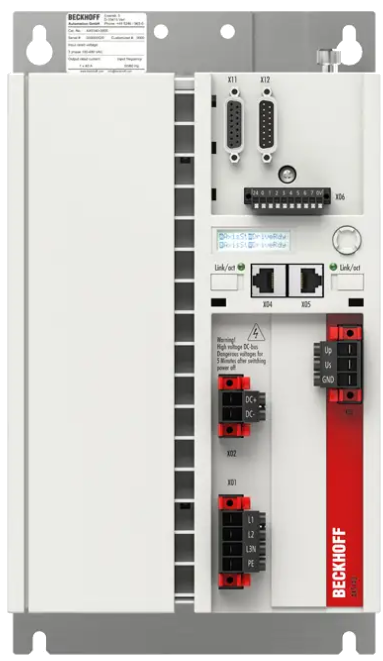
\includegraphics[width=150pt]{AX5140}
	\label{fig:AX5140}
	\caption{De \gls{AX5140} motordrive \cite{web:AX5140Drive}}
\end{figure}

\newpage

\subsection{Eisen}

Hieronder staan de belangrijkste eisen van de testopstelling van dit onderzoek. Voor alle eisen wordt doorverwezen naar het SRD bestand van de testopstelling (bijlage \ref{sec:TestKastSRD}).


	\section{Theoretisch Kader} \label{sec:TheoretischKader}

In dit hoofdstuk wordt de theorie achter de motordrive en de testprotocollen uitgelegd.

\subsection{Motor Testen}

Voorheen werden de spindels die getest werden op de testkast alleen bekeken of deze draaiden en of deze niet te veel trilden. Hierbij werden geen meetgegevens gekwantifiseerd, waardoor er eigenlijk niet veel gezegd kan worden over de staat van de motor met duidelijke meetgegevens. Het zou voor de klant, maar ook voor Voortman, toegevoegde waarde hebben om meetgegevens van de motor te kwantifiseren en deze ook statistisch te beoordelen in een testrapport. Voortman kan op deze manier bewijzen dat de spindel weer correct werkt en in wat voor staat de spindel zich momenteel bevindt.

\subsubsection{Fast Fourier Transformation}

Veel motortesten maken gebruik van een Fourier transformatie om op deze manier iets te kunnen zeggen over het frequentiedomein van de meetgegevens. De Discrete Fourier Transform (\gls{DFT}) converteert een eindige reeks van op een gelijke afstand geplaatste reeks van samples van dezelfde lengte van de discrete-time Fourier transformatie (\gls{DTFT}), wat een frequentiefunctie met complexe getallen is. De \gls{DFT} is een frequentiedomeinrepresentatie van de originele invoerreeks (figuur \ref{fig:FourierTransform}).

\begin{figure}[h]
	\centering
	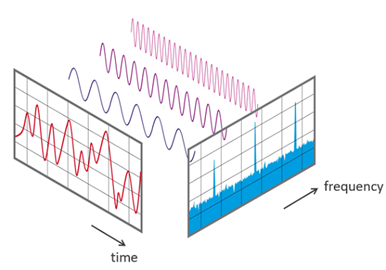
\includegraphics[width=300pt]{FourierTransform}
	\label{fig:FourierTransform}
	\caption{Fourier Transformatie \cite{web:FFT}}
\end{figure}

\newpage

De formule voor de \gls{DFT} is als volgt:

\begin{equation}
	X_k = \sum_{n=0}^{N-1}X_n e^{-i2\pi\frac{k}{N}n}
\end{equation}

Echter kan deze formule erg intensief zijn bij een hoog aantal samples daarom is het beter om een \gls{FFT} te gebruiken zoals het Radix-2 algoritme die het aantal berekeningen aanzienlijk verminderd \cite{web:FFT}:

\begin{equation}
	X_k = {\sum_{m=0}^{\frac{N}{2}-1}X_{2m}e^{-\frac{2\pi i}{N}(2m)k}} + {\sum_{m=0}^{\frac{N}{2}-1}X_{2m+1}e^{-\frac{2\pi i}{N}(2m+1)k}}
\end{equation}

Het idee achter het Radix-2 algoritme is dat eerst alle even getallen berekend worden en hierna de oneven getallen waarna de resultaten gecombineerd worden. Vervolgens kan dit recursief worden berekend. De enige eis hiervan is dat de sample set grootte een macht van 2 moet zijn \cite{web:Radix-2FFT}.

\subsubsection{Lager schade detectie}

De meeste gevallen van motorstoringen komen door slijtage of schade aan de lagers. Lagerschade kan worden gedetecteerd onder andere door het meten van de trillingen van de motor of spindel. Hierbij kan men vier frequentie pieken berekenen in de \gls{FFT} van de trillingen van de spindel waardoor de oorzaak van de schade of de staat van de lager kan worden bepaaldt. Lager schade vormt zich in vier fasen, in de een na laatste fase zullen de berekende pieken zich vormen. Het vervangen van de lager is op dat moment noodzakelijk aangezien de lager het uiteindelijk zal begeven in de laatste fase \cite{web:BearingFault}. Voor meer informatie over deze fasen zie bijlage \ref{sec:LiteratuurOnderzoek} hoofdstuk 6.


\begin{figure}[h]
	\centering
	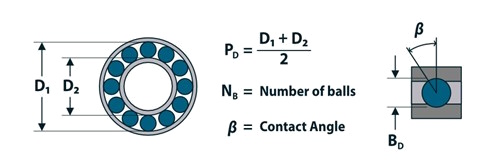
\includegraphics[width=350pt]{LagerSchade}
	\label{fig:LagerSchade}
	\caption{Lager schade herkennen door trillingen \cite{web:BearingFault}}
\end{figure}

\begin{enumerate}
	\item \textbf{Balls Pass Frequency Outer Race (\gls{BPFO})} Deze frequentie komt overeen met het aantal kogels dat door een bepaald punt van de buitenring gaat bij elke volledige draai.
	
	\begin{equation}
		BPFO = RPM\frac{N_b}{2}(1-\frac{B_D}{P_D}\cos\cos\beta)
	\end{equation}
	\newpage
	
	\item \textbf{Ball Pass Frequency Inner Race (\gls{BPFI})} Deze frequentie staat gelijk aan de binnenringstoringsfrequentie. Deze frequentie ontstaat doordat de kogels of rollers langs een bepaald punt komen bij elke rotatie.
	
	\begin{equation}
		BPFI = RPM\frac{N_b}{2}(1-\frac{B_D}{P_D}\cos \cos \beta)
	\end{equation}
	
	\item \textbf{Ball Spin Frequency (\gls{BSF})} Deze frequentie komt overeen met het aantal omwentelingen dat een lager kogel of rol maakt elke keer wanneer de as een volledige draai heeft gemaakt.
	
	\begin{equation}
		BSF = RPM\frac{P_D}{B_D}[1-(\frac{B_D}{P_D} \cos \cos \beta)^2]
	\end{equation}
	
	\item \textbf{Fundamental Train Frequency (\gls{FTF})} Deze frequentie komt overeen met het aantal omwentelingen die de lager kooi maakt bij elke volledige draai.
	
	\begin{equation}
		FTF=RPM\frac{1}{2}(1-\frac{B_D}{P_D} \cos \cos \beta)
	\end{equation}
\end{enumerate}

In figuur \ref{fig:LagerStage3} is een voorbeeld te zien hoe de berekende pieken te zien zouden kunnen zijn wanneer een lager in stage 3 is van zijn slijtage.

\begin{figure}[h]
	\centering
	
	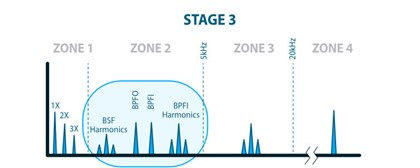
\includegraphics[width=400pt]{LagerStage3}
	
	\label{fig:LagerStage3}
	\caption{Berekende frequentie pieken in een \gls{FFT} van de trillingen \cite{web:BearingFault}}
\end{figure}

\newpage

\subsubsection{Rotor Excentriciteit}

Excentriciteit in de rotor zorgt ongeveer voor 12\% tot 16\% van alle motor storingen \cite{MotorExcenttriciteit}. Er zijn bij rotor excentriciteit twee smaken:

\begin{enumerate}
	\item \textbf{Dynamische excentriciteit} hierbij veranderd de afstand tussen de stator en de rotor constant waardoor er onbalans en trillingen kunnen ontstaan. Oorzaken hiervan kunnen zijn versleten lagers, mechanische speling of een kromme rotorstang.
	
	\item \textbf{Statische excentriciteit} hierbij is de rotor niet in het midden geplaatst van de stator. De afstand tussen de rotor en stator is hierbij constant. Statische excentriciteit zal zorgen voor ongelijke magnetische krachten wat weer zal resulteren in extra energieverbruik en meer slijtage in de lagers.
\end{enumerate}


	\section{Software Ontwerp en Implementatie} \label{sec:Implementatie}
	\section{Uitbreidingen en Verbeteringen} \label{sec:Uitbreidingen}
	\section{Testen en Resultaten}

	\section{Conclusie en Aanbevelingen}
	\section{Reflectie}
	% Referenties zijn te vinden in References.bib

\bibliographystyle{ieeetran}
\bibliography{../GeneralTeX/References}
	\appendix

\section{Bijlage: Testkast SRD} \label{sec:TestKastSRD}

\href{run:TestkastSRD.pdf}{TestkastSRD.pdf}


\end{document}